\section{Question 7}
We apply PCA and Isomap algorithms \cite{anowar2021conceptual} to reduce the dimension of the given dataset from 10 to 3.
The KMeans clustering performance based on silhouette score is calculated for the original dataset and reduced dataset accross 50 clusters.
The result is presented as Figure \ref{Fig: Sil-dim3}.
As can be see, the original dataset have the lowest Silhouette score overall, thus the datasets with reduced dimension have better performance.
It is noticable that the Isomap algorithm can achive better silhouette score compared to PCA.

\begin{figure}
    \centering
    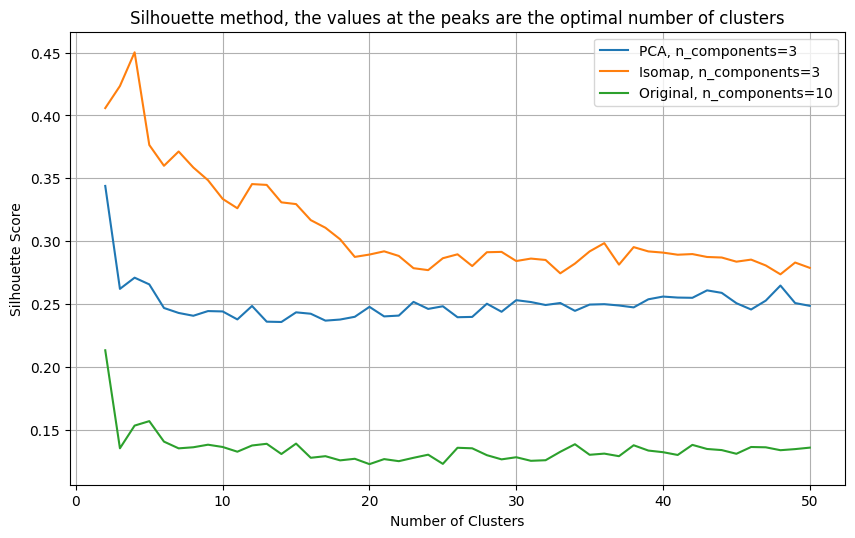
\includegraphics[width=\textwidth]{Appendices/Sil-Dim3.png}
    \caption{Silhouette score for PCA and Isomap reduced dataset, compared to the original}
    \label{Fig: Sil-dim3}
\end{figure}